\documentclass[12pt,fullpage,a4paper,titlepage,oneside]{report}

% Para fazer o contador de figuras ser por documento
\usepackage{chngcntr}
\counterwithout{figure}{chapter}
\counterwithout{table}{chapter}

% Para portugues
\usepackage[brazil]{babel}
\usepackage[utf8]{inputenc}
\usepackage[T1]{fontenc}

\usepackage{setspace} % For doublespacing
%\usepackage{booktabs} % for making better tables
\usepackage[pdftex]{graphicx} % For inserting figures
% \usepackage[draft]{graphicx} % Rascunho
\usepackage[round,sort]{natbib} % For better bibliography

% Mathematical Symbols and fonts
\usepackage{amssymb,amsmath} 
% Define vector commands
\providecommand{\abs}[1]{\lvert#1\rvert}
\providecommand{\norm}[1]{\lVert#1\rVert}
\newcommand{\opt}[1]{\tilde{#1}}
\newcommand{\est}[1]{\hat{#1}}
\newcommand{\vect}[1]{\bar{#1}}
\newcommand{\mat}[1]{\bar{\bar{#1}}}

% Fix the margins so that they are bit smaller
\usepackage[a4paper]{geometry}
\geometry{verbose,tmargin=3cm,bmargin=3cm,lmargin=3cm,rmargin=2.5cm}

% Make the fancy header
\usepackage{fancyhdr}
\pagestyle{fancy}
\renewcommand{\chaptermark}[1]{\markboth{\thechapter.\ #1}{}}
\renewcommand{\sectionmark}[1]{\markright{\thesection\ #1}}
\fancyhf{} % delete current header and footer
\rhead{\bfseries\thepage}
\lhead{\bfseries\leftmark}
\cfoot{}
\addtolength{\headheight}{15.5pt} % space for the rule
\fancypagestyle{plain}{
    \fancyfoot{} 
    \renewcommand{\headrulewidth}{0pt} % and the line
    \rhead{\bfseries\thepage}
    \lhead{}
}

% Information
\title{\bf TÓPICOS DE \\[0.8cm] INVERSÃO EM GEOFÍSICA \vspace{1cm}}
\author{Vanderlei Coelho de Oliveira Junior\\[0.3cm]Leonardo Uieda}
\date{\vfill Versão 0.1\\[0.5cm] 2011}

% For pdf hyperlinks
\usepackage[pdftex]{hyperref}
\hypersetup{colorlinks=true}
\hypersetup{citecolor=blue}
\hypersetup{pdftitle={Tópicos de inversão em geofísica}}
\hypersetup{pdfauthor={Vanderlei Coelho de Oliveira Junior \& Leonardo Uieda}}
% For making a print without color links
%\hypersetup{linkcolor=black,citecolor=black,filecolor=black,urlcolor=black}

\begin{document}
    \maketitle
    \newpage
    \thispagestyle{empty}
\clearpage

\noindent {\Large \bf Tópicos inversão em geofísica}
\\[1cm]
\noindent Copyright \copyright\ 2011
Vanderlei Coelho de Olivera Junior and Leonardo Uieda
\\[0.5cm]
\noindent Licensa blablabla

    \pagenumbering{roman}
    \doublespacing
    \chapter*{Prefácio}
\addcontentsline{toc}{chapter}{Prefácio}

    Meh

    \tableofcontents
    \newpage
    \pagenumbering{arabic}
    \chapter{Introdução}

\indent Em ciências aplicadas, ao nos depararmos com uma determinada coisa a ser
estudada, a pergunta imediata é: como estudar tal coisa? Em problemas geofísicos,
essa coisa é, em geral, um sistema físico. O procedimento científico utilizado
para estudá-lo começa com a realização de observações (medições) de uma
determinada grandeza física que, supostamente, seja causada pelo sistema físico.
\\
\indent Exemplos de sistemas físicos encontrados na geofísica são:

\begin{itemize}
    \item{Propagação de ondas elásticas: sísmica (Figura \ref{system-seismic})}
    \item{Gravitação: gravimetria (Figura \ref{system-grav})}
    \item{Difusão de correntes elétricas: SEV (Figura \ref{system-sev})}
\end{itemize}

\begin{figure}
    \centering
    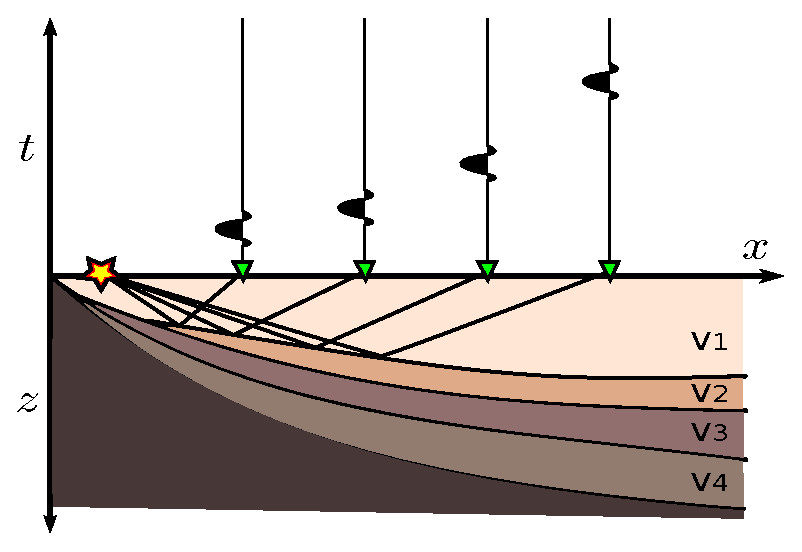
\includegraphics[scale=1]{../figs/system-seismic.eps}
    \caption{Exemplo de sistema físico que caracteriza uma aquisição sísmica.
        Neste caso o sistema envolve ondas sísmicas que se propagam em meios com
        diferentes velocidades. A grandeza física que podemos observar (medir)
        é o deslocamento dos sismômetros (neste caso somente na vertical).
        Estas observações são tipicamente dispostas em um sismograma.}
    \label{system-seismic}
\end{figure}

\begin{figure}
    \centering
    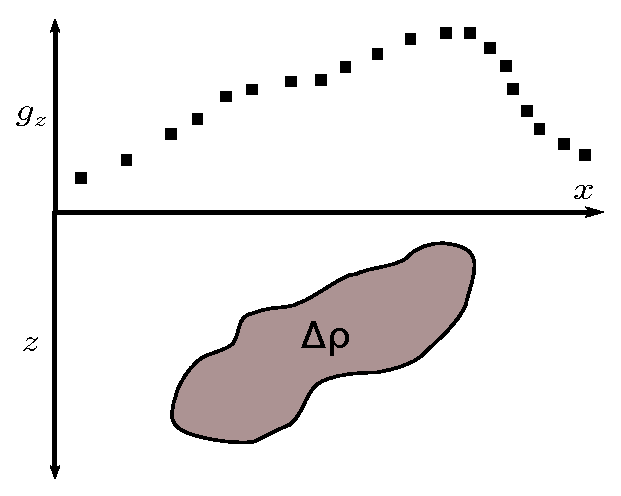
\includegraphics[scale=1]{../figs/system-grav.eps}
    \caption{Exemplo de sistema físico que caracteriza um levantamento
        gravimétrico. Neste caso o sistema envolve o efeito gravitacional
        causado por um contraste de densidade anômalo. A grandeza física que
        podemos observar (medir) é a anomalia da gravidade.}
    \label{system-grav}
\end{figure}

\begin{figure}
    \centering
    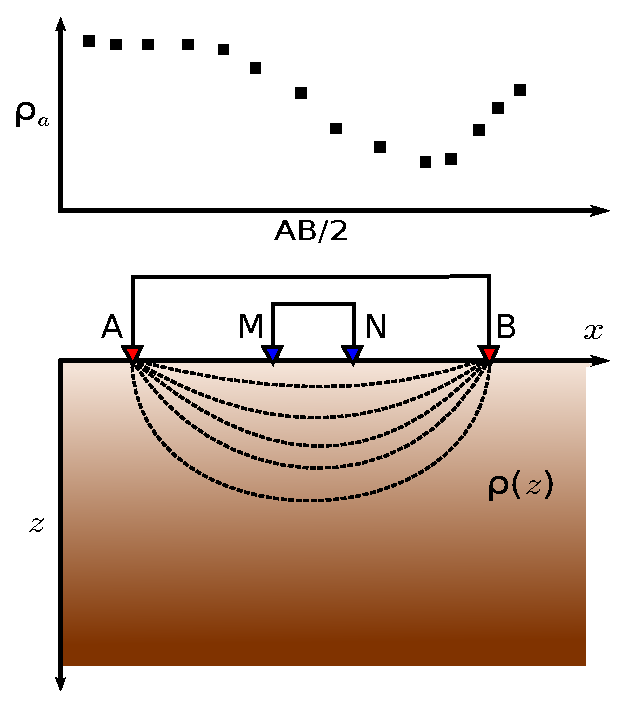
\includegraphics[scale=1]{../figs/system-sev.eps}
    \caption{Exemplo de sistema físico que caracteriza uma sondagem elétrica
        vertical (SEV). Neste caso o sistema envolve a condução de correntes
        elétricas em meios com diferentes resistividades elétricas ($\rho$).
        A grandeza física que podemos observar (medir) é diferência de potencial
        elétrico entre os eletrodos M e N. Esta grandeza é geralmente convertida
        para resistividade aparente ($\rho_a$).}
    \label{system-sev}
\end{figure}

\indent Uma vez que não conhecemos o sistema físico, a única coisa que temos são as
observações (dados observados). Contudo, embora o sistema físico seja
desconhecido, alguma informação adicional (em geral proporcionada pela geologia)
nos fornece um conjunto de hipóteses.
\\
Exemplos de hipóteses (sem dados observados e nem dados preditos)
\\
\indent Isso nos leva a seguinte pergunta: como testar se as observações podem ser
explicadas por uma determinada hipótese? Para responder esta pergunta,
precisamos ser capazes de calcular os dados preditos pela hipótese em questão.
\\
Exemplos de hipóteses e os respectivos dados preditos (sem dados observados)
\\
\indent Matematicamente, isso significa que precisamos encontrar uma função que
relaciona a hipótese aos dados preditos.

\begin{figure}[!htb]
  \centering
    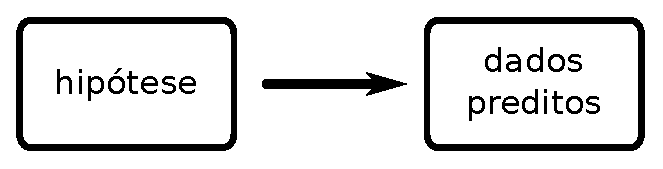
\includegraphics[scale=1]{../figs/hipotese-preditos.eps}
  %\caption{}
  \label{hipotese-preditos}
\end{figure}

Uma função é descrita em termos de parâmetros:
\\
Exemplos de funções
\\
\indent Portanto, calcular os dados preditos por uma determinada hipótese significa
encontrar uma função $f$ tal que:

\[
\text{dados preditos} = f(\text{hipótese}).
\]

\indent Para tanto, é preciso descrever a hipótese em termos de parâmetros
(parametrização), isto é:

\[
\text{dados preditos} = f(\text{parâmetros}).
\]

Exemplos de parametrização das hipóteses
\\
\indent O raciocínio desenvolvido acima nos permite definir um importante conceito:

\begin{quotation}
{\tt Estabelecer a relação funcional entre parâmetros (que descrevem uma hipótese)
e dados preditos é o que se co\-nhe\-ce como {\bf pro\-ble\-ma direto}.}
\end{quotation}

\indent Nesse sentido, dado um conjunto de parâmetros, é possível calcular os dados
preditos e isso nos permite testar se uma hipótese é capaz de explicar os dados
observados. Esse teste é feito por meio da comparação entre os dados observados
e os dados preditos por uma determinada hipótese. Se os dados preditos
reproduzem os dados observados, pode-se dizer que a hipótese explica os dados
observados e, portanto, é válida.
\\
Exemplos de hipóteses com os respectivos dados preditos, parâmetros e os dados observados
\\
\indent Nesse contexto, é possível podemos definir os seguintes conceitos importantes:

\begin{quotation}
{\tt Fornecer os parâmetros e comparar os respectivos dados preditos com os dados
observados é o que se conhece como {\bf mo\-de\-la\-gem direta}.}
\end{quotation}

e

\begin{quotation}
{\tt Estimar os parâmetros automaticamente, de forma que os dados preditos sejam os
mais próximos possíveis aos dados observados, é conhecido como {\bf problema inverso}.}
\end{quotation}

Figuras das setinhas

    \chapter{Formulação matemática do problema inverso}

Dado um conjunto de $N$ observações, feitas em diferentes posições, tempos, etc.,
de\-fi\-ni\-mos um {\it vetor de dados observados}

\begin{equation}
\vect{d}^{\thinspace o} =
    \begin{bmatrix}
    d_1^{\thinspace o} \\
    d_2^{\thinspace o} \\
    \vdots \\
    d_N^{\thinspace o}
    \end{bmatrix},
\end{equation}

\noindent em que $d_i^{\thinspace o}$, $i = 1, 2, 3, \dotsc, N$, é o dado
observado na $i$-ésima posição, tempo, etc.
De forma análoga, definimos um {\it vetor de dados preditos}

\begin{equation}
\vect{d}^{\thinspace p} =
    \begin{bmatrix}
    d_1^{\thinspace p} \\
    d_2^{\thinspace p} \\
    \vdots \\
    d_N^{\thinspace p}
    \end{bmatrix},
\end{equation}

\noindent em que $d_i^{\thinspace p}$, $i = 1, 2, 3, \dotsc, N$, é o dado predito
calculado na mesma posição, tempo, etc., que o $i$-ésimo dado observado.
Continuando no espírito de definição de vetores, definimos também um vetor que
agrupa todos os $M$ parâmetros, denominado {\it vetor de parâmetros}

\begin{equation}
\vect{p} =
    \begin{bmatrix}
    p_1 \\
    p_2 \\
    \vdots \\
    p_M
    \end{bmatrix},
\label{eq:param_vect}
\end{equation}

\noindent em que $p_j$, $j = 1, 2, 3, \dotsc, M$, é o $j$-ésimo parâmetro.
\\
\indent Como vimos no Capítulo \ref{chap:intro}, os dados preditos são descritos
por uma função dos parâmetros, ou seja,

\begin{equation}
d^{\thinspace p}_i = f_i(\vect{p})\thinspace.
\label{eq:fi}
\end{equation}

\noindent Desta forma, podemos dizer que o vetor de dados preditos é uma função
dos parâmetros

\begin{equation}
\vect{d}^{\thinspace p}= \vect{f}(\vect{p}) =
    \begin{bmatrix}
    f_1(\vect{p}) \\
    f_2(\vect{p}) \\
    \vdots \\
    f_N(\vect{p})
    \end{bmatrix}.
\label{eq:dados_preditos}
\end{equation}

\indent O problema inverso consiste em encontrar um vetor de parâmetros $\vect{p}$
que produza os dados preditos mais próximos possívies dos dados observados.
Para determinar a ``proximidade'' entre os dados observados e os dados preditos,
é necessário quantificar a distância entre eles.
Isto é feito em termos da norma do {\it vetor de resíduos}

\begin{equation}
\vect{r} = \vect{d}^{\thinspace o} - \vect{f}(\vect{p}),
\end{equation}

\noindent em que $\vect{d}^{\thinspace o}$ é o vetor de {\it dados observados}
e $\vect{f}(\vect{p})$ é o vetor de {\it dados preditos}.
\\
\indent Para quantificar a distância entre os dados observados e os dados
preditos utiliza-se, usualmente, o quadrado da
norma quadrática (também conhecida como norma $\ell_2$ ou norma Euclidiana)
do vetor de resíduos

\begin{equation}
\norm{\vect{r}}_2^2 =
    \sum\limits_{i=1}^N \left[d^{\thinspace o}_i - f_i(\vect{p})\right]^2 \, .
\label{eq:norma_l2}
\end{equation}

\noindent Esta equação é também uma função escalar
dos parâmetros. Assim sendo, definimos uma função $\phi(\vect{p})$, chamada de
{\it função do ajuste}, como

\begin{equation}
\phi(\vect{p}) = \norm{\vect{r}}_2^2 =
    \sum\limits_{i=1}^N \left[d^{\thinspace o}_i - f_i(\vect{p})\right]^2 \, .
\label{eq:ajuste_sum}
\end{equation}

\indent Lembramos que o quadrado da norma Euclidiana de um vetor é igual ao
produto escalar do vetor com ele mesmo, ou seja,

\begin{equation}
\norm{\vect{r}}_2^2 = \vect{r} \cdot \vect{r} =
    r_1r_1 + r_2r_2 + \dotsb + r_Nr_N \thinspace .
\label{eq:dotprod}
\end{equation}

\noindent Como o vetor $\vect{r}$ é um {\it vetor coluna} (matriz com uma
coluna), podemos escrever o produto escalar da equação \ref{eq:dotprod} como

\begin{equation}
\vect{r} \cdot \vect{r} = \vect{r}^T \vect{r} =
    \begin{bmatrix}
        r_1 & r_2 & \ldots & r_N
    \end{bmatrix}
    \begin{bmatrix}
        r_1 \\ r_2 \\ \vdots \\ r_N
    \end{bmatrix} .
\label{eq:vectdotprod}
\end{equation}

\noindent Dessa forma podemos reescrever a função do ajuste (equação
\ref{eq:ajuste_sum}) como

\begin{equation}
\phi(\vect{p}) = \vect{r}^T \vect{r} =
    \left[\vect{d}^{\thinspace o} - \vect{f}(\vect{p})\right]^T
    \left[\vect{d}^{\thinspace o} - \vect{f}(\vect{p})\right] .
\label{eq:ajuste}
\end{equation}

\indent Neste ponto é importante ressaltar o seguinte conceito:

\begin{quote}
{\tt A {\bf função do ajuste} é uma função escalar que
quantifica a dis\-tân\-cia entre os dados observados e os dados preditos para um
de\-ter\-mi\-na\-do vetor de parâmetros $\vect{p}$.}
\end{quote}

\indent Perante este conceito, o problema inverso consiste em determinar um
vetor $\opt{p}$ que minimiza a função do ajuste $\phi(\vect{p})$. 
Matematicamente, isso equivale a encontrar o vetor $\opt{p}$ tal que o gradiente
da função $\phi(\vect{p})$ avaliado em $\opt{p}$ seja igual ao vetor nulo.
Este vetor $\opt{p}$ é um {\it ponto extremo} da função
$\phi(\vect{p})$.
\\
\indent O gradiente da função $\phi(\vect{p})$, avaliado em um $\vect{p}$ qualquer,
é um vetor $M$-dimensional definido como (ver Apêndice \ref{chap:opmat})

\begin{equation}
\vect{\nabla} \phi(\vect{p}) =
    \begin{bmatrix}
        \dfrac{\partial \phi(\vect{p})}{\partial p_1} \vspace{0.3cm}\\
        \dfrac{\partial \phi(\vect{p})}{\partial p_2}\\
        \vdots \\
        \dfrac{\partial \phi(\vect{p})}{\partial p_M}
    \end{bmatrix} ,
\label{eq:gradphi_partial}
\end{equation} 

\noindent em que $\vect{\nabla}$ é o operador gradiente (Apêndice \ref{chap:opmat}).
A partir da equação \ref{eq:ajuste}, a expressão para o $i$-ésimo elemento do
vetor gradiente é

\begin{equation}
\begin{split}
\dfrac{\partial \phi(\vect{p})}{\partial p_i} &=
    \dfrac{\partial}{\partial p_i}\left\{
        \left[\vect{d}^{\thinspace o} - \vect{f}(\vect{p})\right]^T
        \left[\vect{d}^{\thinspace o} - \vect{f}(\vect{p})\right]
    \right\} \\[0.5cm]
    &= 
    \underbrace{
    \left\{-\dfrac{\partial\vect{f}(\vect{p})}{\partial p_i}^T
            \left[\vect{d}^{\thinspace o} - \vect{f}(\vect{p})\right]
    \right\}}_{\text{escalar}}
    +
    \underbrace{
    \left\{-\left[\vect{d}^{\thinspace o} - \vect{f}(\vect{p})\right]^T            
            \dfrac{\partial\vect{f}(\vect{p})}{\partial p_i}
    \right\}}_{\text{escalar}}
\end{split} .
\label{eq:del_phi_del_pi}
\end{equation}

\indent Lembrando que o transposto de um escalar é igual a ele mesmo, podemos
tomar o transposto do segundo termo do lado direito da equação
\ref{eq:del_phi_del_pi}, obtendo

\begin{equation}
\dfrac{\partial \phi(\vect{p})}{\partial p_i} = 
    -2\dfrac{\partial\vect{f}(\vect{p})}{\partial p_i}^T
    \left[\vect{d}^{\thinspace o} - \vect{f}(\vect{p})\right],
\label{eq:del_phi_del_pi_simple}
\end{equation}

\noindent em que $\dfrac{\partial\vect{f}(\vect{p})}{\partial p_i}$ é um vetor
$N$-dimensional (ver Apêndice \ref{chap:opmat}) dado por

\begin{equation}
\dfrac{\partial\vect{f}(\vect{p})}{\partial p_i} =
    \begin{bmatrix}
        \dfrac{\partial f_1(\vect{p})}{\partial p_i} \vspace{0.3cm}\\
        \dfrac{\partial f_2(\vect{p})}{\partial p_i}\\
        \vdots \\
        \dfrac{\partial f_N(\vect{p})}{\partial p_i}
    \end{bmatrix}.
\label{eq:del_f_del_pi}
\end{equation}

\indent Substituindo as equações \ref{eq:del_phi_del_pi_simple} e
\ref{eq:del_f_del_pi} na expressão do gradiente (equação \ref{eq:gradphi_partial})
obtemos

\begin{equation}
\begin{split}
\vect{\nabla} \phi(\vect{p}) &=
        \begin{bmatrix}
            -2\dfrac{\partial\vect{f}(\vect{p})}{\partial p_1}^T
                \left[\vect{d}^{\thinspace o} - \vect{f}(\vect{p})\right]
                \vspace{0.3cm} \\
            -2\dfrac{\partial\vect{f}(\vect{p})}{\partial p_2}^T
                \left[\vect{d}^{\thinspace o} - \vect{f}(\vect{p})\right]\\
            \vdots \\
            -2\dfrac{\partial\vect{f}(\vect{p})}{\partial p_M}^T
                \left[\vect{d}^{\thinspace o} - \vect{f}(\vect{p})\right]
        \end{bmatrix}
    \\[0.5cm] &=
        -2
        \begin{bmatrix}
            \dfrac{\partial\vect{f}(\vect{p})}{\partial p_1}^T\vspace{0.3cm} \\
            \dfrac{\partial\vect{f}(\vect{p})}{\partial p_2}^T \\
            \vdots \\
            \dfrac{\partial\vect{f}(\vect{p})}{\partial p_M}^T
        \end{bmatrix}
        \left[\vect{d}^{\thinspace o} - \vect{f}(\vect{p})\right].
\end{split}
\label{eq:gradphi_partial_f}
\end{equation}

\noindent Por fim, o gradiente da função do ajuste $\phi(\vect{p})$ pode ser
escrito como

\begin{equation}
\vect{\nabla} \phi(\vect{p}) = -2\mat{G}(\vect{p})^T
    \left[\vect{d}^{\thinspace o} - \vect{f}(\vect{p})\right].
\label{eq:gradphi}
\end{equation}

\noindent em que 

\begin{equation}
\mat{G}(\vect{p}) = 
\begin{bmatrix}
    \dfrac{\partial\vect{f}(\vect{p})}{\partial p_1} &
    \dfrac{\partial\vect{f}(\vect{p})}{\partial p_2} &
    \ldots &
    \dfrac{\partial\vect{f}(\vect{p})}{\partial p_M}
\end{bmatrix}
=
\begin{bmatrix}
    \dfrac{\partial f_1(\vect{p})}{\partial p_1} &
        \dfrac{\partial f_1(\vect{p})}{\partial p_2} &
        \ldots &
        \dfrac{\partial f_1(\vect{p})}{\partial p_M}
    \vspace{0.3cm}\\
    \dfrac{\partial f_2(\vect{p})}{\partial p_1} &
        \dfrac{\partial f_2(\vect{p})}{\partial p_2} &
        \ldots & 
        \dfrac{\partial f_2(\vect{p})}{\partial p_M}
    \\
    \vdots & \vdots & \ddots & \vdots
    \\
    \dfrac{\partial f_N(\vect{p})}{\partial p_1} &
        \dfrac{\partial f_N(\vect{p})}{\partial p_2} &
        \ldots & 
        \dfrac{\partial f_N(\vect{p})}{\partial p_M}        
\end{bmatrix}.
\label{eq:jacobian}
\end{equation}

\noindent A matriz $\mat{G}(\vect{p})$ de dimensão $N \times M$ é a
{\it matriz Jacobiana} de $\vect{f}(\vect{p})$.

\begin{quote}
{\tt Em problemas inversos, essa matriz $\mat{G}$ é comumente denominada
{\bf matriz de sensibilidade}, uma vez que o $i$-ésimo elemento de sua $j$-ésima
coluna expressa a sensibilidade do $i$-ésimo dado pre\-di\-to em re\-la\-ção à variações
do $j$-ésimo parâmetro.}
\end{quote}

\indent As equações \ref{eq:gradphi} e \ref{eq:jacobian} mostram que o gradiente
da função do ajuste $\phi(\vect{p})$ depende do vetor de dados preditos
$\vect{f}(\vect{p})$ (equação \ref{eq:dados_preditos}) e sua derivada em relação
aos parâmetros $\vect{p}$.
Sendo assim, a função $f$ que relaciona os parâmetros aos dados preditos determina
o comportamento do gradiente de $\phi(\vect{p})$.
Nas próximas seções analisaremos os casos em que a função $f$ é linear ou
não-linear em relação aos parâmetros.
Essa análise nos permitirá compreender a influência da função $f$ na busca pelo
vetor de parâmetros $\opt{p}$ que minimiza a função $\phi(\vect{p})$.

\section{Problemas lineares}

Se a função $f_i(\vect{p})$ (equação \ref{eq:fi}), que relaciona o vetor de
parâmetros $\vect{p}$ ao $i$-ésimo dado predito, for uma combinação linear dos
parâmetros, ela terá a seguinte forma

\begin{equation}
f_i(\vect{p}) = g_{i1}p_1 + g_{i2}p_2 + \dotsb + g_{iM}p_M + b_i \thinspace ,
\label{eq:comb_linear}
\end{equation}

\noindent em que $g_{ij}$, $j = 1, 2, \cdots, M$, e $b_i$ são constantes.
Portanto, a derivada de $f_i(\vect{p})$ em relação ao $j$-ésimo parâmetro
$p_j$ é dada por

\begin{equation}
\dfrac{\partial f_i(\vect{p})}{\partial p_j} = g_{ij} \thinspace ,
\end{equation}

\noindent que não depende dos parâmetros. Para um conjunto de $N$ dados, o vetor
de dados preditos tem a seguinte forma

\begin{equation}
\vect{f}(\vect{p}) = \mat{G}\vect{p} + \vect{b} \thinspace ,
\label{eq:f_igual_Gp}
\end{equation}

\noindent sendo $\mat{G}$ a matriz de sensibilidade (equação \ref{eq:jacobian})
e $\vect{b}$ um vetor de constantes.
Substituindo a expressão acima no gradiente da função do ajuste (equação
\ref{eq:gradphi}), chegamos a

\begin{equation}
\vect{\nabla}\phi(\vect{p}) = -2\mat{G}^T \left(\vect{d}^{\thinspace o} -
    \mat{G}\vect{p} - \vect{b} \right).
\end{equation}

\indent Seja $\opt{p}$ o vetor que minimiza a função $\phi(\vect{p})$, o
gradiente desta função avaliado em $\opt{p}$ é igual ao vetor nulo.
Isto nos leva ao sistema de equações

\begin{equation}
\mat{G}^T\mat{G}\opt{p} = \mat{G}^T\left(\vect{d}^{\thinspace o} - \vect{b} \right).
\label{eq:sistema_normal}
\end{equation}

\noindent Este sistema é conhecido como {\it sistema de equações normais}. A
solução para este sistema é

\begin{equation}
\opt{p} = (\mat{G}^T\mat{G})^{-1} \mat{G}^T
    \left(\vect{d}^{\thinspace o} - \vect{b} \right),
\label{eq:estimador_mq}
\end{equation}

\noindent que é conhecido como {\it estimador de mínimos quadrados}.
\\
\indent As equações \ref{eq:sistema_normal} e \ref{eq:estimador_mq} mostram que 
o vetor $\opt{p}$ que minimiza a função $\phi(\vect{p})$ pode ser
obtido diretamente a partir da matriz $\mat{G}$ e dos vetores $\vect{b}$ e
$\vect{d}^{\thinspace o}$. Isto caracteriza um {\it problema inverso linear}.

\section{Problemas não-lineares}

Nesta seção analisaremos o caso em que a função $f_i(\vect{p})$
(equação \ref{eq:fi}) não é uma combinação linear dos parâmetros.
Neste caso, a derivada de $f_i(\vect{p})$ em relação aos parâmetros também será
uma função dos parâmetros.
Logo, dependendo das características da função $f_i(\vect{p})$, o gradiente da
função do ajuste $\phi(\vect{p})$ pode ser nulo para mais de um valor de
$\vect{p}$.
Em outras palavras, a função $\phi(\vect{p})$ pode possuir
vários pontos extremos além daquele em que esta função seja mínima.
Por esta razão, o cálculo do vetor $\opt{p}$ que minimiza a função do ajuste deve
ser feito de forma iterativa.
Isto difere do problema inverso linear e caracteriza um {\it problema inverso
não-linear}.
\\
\indent A busca pelo vetor $\opt{p}$ que minimiza uma determinada função faz
parte de uma área da matemática conhecida como {\it otimização}, dentro da qual
existem diversos métodos (KELLEY, 1999).
O procedimento padrão para realizar esta busca de forma iterativa é começar com
uma determinada aproximação inicial $\vect{p}_0$ e calcular uma correção
$\Delta\vect{p}$.
Esta correção é então aplicada à aproximação inicial dando origem a um novo vetor
$\vect{p}_1$.
Este novo vetor serve como aproximação inicial para o cálculo de um segundo
vetor $\vect{p}_2$, e assim sucessivamente.
O processo termina quando é encontrado um vetor $\est{p}$ que seja próximo ao
vetor $\opt{p}$ que minimiza a função em questão.
Em geral, não se tem garantia de que o vetor $\est{p}$ seja igual ao vetor
$\opt{p}$.
\\
\indent Dentre os vários métodos existentes, apresentaremos a seguir aquele
conhecido como método de Gauss-Newton.
O procedimento para calcular a correção $\Delta\vect{p}$ começa com a
expansão em série de Taylor da função a ser minimizada, neste caso $\phi(\vect{p})$.
A expansão é feita até segunda ordem e em torno da aproximação inicial $\vect{p}_0$
(ver Apêndice \ref{chap:opmat})

\begin{equation}
\vect{p} =  \vect{p}_0 + \Delta\vect{p} \thinspace ,
\end{equation}

\begin{equation}
\phi(\vect{p}_0 + \Delta\vect{p}) \approx \phi(\vect{p}_0) +
    \vect{\nabla}\phi(\vect{p}_0)^T\Delta\vect{p} +
    \dfrac{1}{2}\Delta\vect{p}^T\mat{\nabla}\phi(\vect{p}_0)\Delta\vect{p}
= \psi(\vect{p}) \thinspace ,
\label{eq:taylor}
\end{equation}

\noindent sendo $\vect{\nabla}\phi(\vect{p}_0)$ o vetor gradiente  e
$\mat{\nabla}\phi(\vect{p}_0)$ a {\it matriz Hessiana} da função $\phi(\vect{p})$,
calculados em $\vect{p}_0$.
\\
\indent A função $\psi(\vect{p})$ (equação \ref{eq:taylor}) é uma aproximação
de segunda ordem para a função $\phi(\vect{p})$ em torno do ponto $\vect{p}_0$.
Tal como no {\it problema inverso linear}, desejamos encontrar um ponto $\est{p}$
que minimiza a função $\psi(\vect{p})$, ou seja, onde seu gradiente é nulo.
O gradiente de $\psi(\vect{p})$ é dado por (ver Apêndice \ref{chap:opmat})

\begin{equation}
\vect{\nabla}\psi(\vect{p}) = \vect{\nabla}\left[
    \phi(\vect{p}_0) +
    \vect{\nabla}\phi(\vect{p}_0)^T\Delta\vect{p} +
    \dfrac{1}{2}\Delta\vect{p}^T\mat{\nabla}\phi(\vect{p}_0)\Delta\vect{p}
    \right] =
    \vect{\nabla}\phi(\vect{p}_0) + \mat{\nabla}\phi(\vect{p}_0)\Delta\vect{p}
    \thinspace .
\end{equation}

\noindent Logo, o incremento $\Delta\vect{p} = \est{p} - \vect{p}_0$, que leva
da aproximação inicial ao ponto $\est{p}$ onde o gradiente de $\psi(\vect{p})$ é
nulo, é a solução do sistema de equações

\begin{equation}
     \mat{\nabla}\phi(\vect{p}_0)\Delta\vect{p} = -\vect{\nabla}\phi(\vect{p}_0)
    \thinspace .
\label{eq:sistema_normal_nlin}
\end{equation}

\indent O cálculo do vetor gradiente de $\phi(\vect{p})$ foi feito anteriormente
(equação \ref{eq:gradphi}), restando então o cálculo da matriz Hessiana
$\mat{\nabla}\phi(\vect{p})$.
Para tanto, deriva-se o $i$-ésimo elemento do vetor gradiente
(equações \ref{eq:gradphi_partial} e \ref{eq:del_phi_del_pi_simple}) em relação
ao $j$-ésimo elemento do vetor de parâmetros $p_j$ (equação \ref{eq:param_vect})

\begin{equation}
\begin{split}
\dfrac{\partial}{\partial p_j}\left(\dfrac{\partial \phi(\vect{p})}{\partial p_i}\right)
&=
\dfrac{\partial}{\partial p_j}\left(
    -2\dfrac{\partial\vect{f}(\vect{p})}{\partial p_i}^T
    \left[\vect{d}^{\thinspace o} - \vect{f}(\vect{p})\right]
    \right)
\\[0.5cm]
&=
\underbrace{
\left( -2\dfrac{\partial^2 \vect{f}(\vect{p})}{\partial p_j \partial p_i}^T
\left[\vect{d}^{\thinspace o} - \vect{f}(\vect{p})\right]
\right)}_{\text{escalar}} +
\underbrace{
\left( 2 \dfrac{\partial\vect{f}(\vect{p})}{\partial p_i}^T
    \dfrac{\partial\vect{f}(\vect{p})}{\partial p_j} \right)}_{\text{escalar}} .
\end{split}
\label{eq:hessian_ij_exact}
\end{equation}

\indent Esta equação \ref{eq:hessian_ij_exact} representa o $j$-ésimo elemento
da $i$-ésima linha da matriz Hessiana (ver Apêndice \ref{chap:opmat}).
No método de Gauss-Newton, o termo envolvendo as segundas derivadas de
$\vect{f}(\vect{p})$ é negligenciado.
Desta forma a equação \ref{eq:hessian_ij_exact} pode ser aproximada por

\begin{equation}
\dfrac{\partial}{\partial p_j}\left(\dfrac{\partial \phi(\vect{p})}{\partial p_i}\right)
\approx 2 \dfrac{\partial\vect{f}(\vect{p})}{\partial p_i}^T
    \dfrac{\partial\vect{f}(\vect{p})}{\partial p_j} \thinspace .
\label{eq:hessian_ij_approx}
\end{equation}

\noindent Sendo assim, matriz Hessiana avaliada em $\vect{p}_0$ é dada por

\begin{equation*}
\mat{\nabla}\phi(\vect{p}_0) \approx
    2
    \begin{bmatrix}
    \dfrac{\partial\vect{f}(\vect{p}_0)}{\partial p_1}^T\dfrac{\partial\vect{f}(\vect{p}_0)}{\partial p_1} &
    \dfrac{\partial\vect{f}(\vect{p}_0)}{\partial p_1}^T\dfrac{\partial\vect{f}(\vect{p}_0)}{\partial p_2} &
    \ldots &
    \dfrac{\partial\vect{f}(\vect{p}_0)}{\partial p_1}^T\dfrac{\partial\vect{f}(\vect{p}_0)}{\partial p_M}
    \vspace{0.3cm}\\
    \dfrac{\partial\vect{f}(\vect{p}_0)}{\partial p_2}^T\dfrac{\partial\vect{f}(\vect{p}_0)}{\partial p_1} &
    \dfrac{\partial\vect{f}(\vect{p}_0)}{\partial p_2}^T\dfrac{\partial\vect{f}(\vect{p}_0)}{\partial p_2} &
    \ldots &
    \dfrac{\partial\vect{f}(\vect{p}_0)}{\partial p_2}^T\dfrac{\partial\vect{f}(\vect{p}_0)}{\partial p_M}
    \\
    \vdots & \vdots & \ddots & \vdots
    \\
    \dfrac{\partial\vect{f}(\vect{p}_0}{\partial p_M}^T\dfrac{\partial\vect{f}(\vect{p}_0)}{\partial p_1} &
    \dfrac{\partial\vect{f}(\vect{p}_0)}{\partial p_M}^T\dfrac{\partial\vect{f}(\vect{p}_0)}{\partial p_2} &
    \ldots &
    \dfrac{\partial\vect{f}(\vect{p}_0)}{\partial p_M}^T\dfrac{\partial\vect{f}(\vect{p}_0)}{\partial p_M}
    \end{bmatrix} ,
\end{equation*}

\noindent ou

\begin{equation}
\mat{\nabla}\phi(\vect{p}_0) \approx
    2
    \begin{bmatrix}
    \dfrac{\partial\vect{f}(\vect{p}_0)}{\partial p_1}^T \vspace{0.3cm}\\
    \dfrac{\partial\vect{f}(\vect{p}_0)}{\partial p_2}^T \\
    \vdots \\
    \dfrac{\partial\vect{f}(\vect{p}_0)}{\partial p_M}^T
    \end{bmatrix}
    \begin{bmatrix}
    \dfrac{\partial\vect{f}(\vect{p}_0)}{\partial p_1} &
    \dfrac{\partial\vect{f}(\vect{p}_0)}{\partial p_2} &
    \ldots &
    \dfrac{\partial\vect{f}(\vect{p}_0)}{\partial p_M}
    \end{bmatrix}
    =
    \mat{G}(\vect{p}_0)^T\mat{G}(\vect{p}_0) \thinspace ,
\label{eq:hessian_approx}
\end{equation}

\noindent em que $\mat{G}(\vect{p}_0)$ é a {\it matriz de sensibilidade}
(equação \ref{eq:jacobian}) avaliada em $\vect{p}_0$.
\\
\indent A partir das equações \ref{eq:gradphi} e \ref{eq:hessian_approx}, o
sistema de equações \ref{eq:sistema_normal_nlin} pode ser escrito como

\begin{equation}
    \mat{G}(\vect{p}_0)^T\mat{G}(\vect{p}_0)\Delta\vect{p} =
        -\mat{G}(\vect{p}_0)^T \left[
            \vect{d}^{\thinspace o} - \vect{f}(\vect{p}_0) \right]
    \thinspace ,
\label{eq:sistema_normal_gaussnewton}
\end{equation}

\noindent em que
\\
\indent A equação \ref{eq:sistema_normal_gaussnewton} descreve o cálculo da correção
$\Delta\vect{p}$ em uma determinada iteração do método Gauss-Newton.



    \chapter{Regularização}

As equações \ref{eq:sistema_normal} do problema inverso linear e
\ref{eq:sistema_normal_nlin} do problema inverso não-linear são
{\it equações normais}.
Estas equações são sistemas lineares cuja matriz é quadrada.
Para que a solução de uma equação normal seja única, é necessário que esta
matriz tenha {\it posto completo}.
Uma condição para que uma matriz tenha posto completo é que todas as suas colunas
(ou linhas) sejam {\it linearmente independentes}.
Esta condição é equivalente a dizer que a matriz possua determinante diferente de
zero.
\\
\indent Em problemas geofísicos, é comum que a matriz do sistema normal possua
determinante próximo de zero. Ou seja, para fins práticos pode-se considerar que
a matriz {\it não} tenha posto completo.
Isto faz com que o problema inverso geofísico seja um problema {\it mal posto}.

\begin{quote}
{\tt Um problema {\bf mal-posto} apresenta, principalmente, {\it instabilidade}
e {\it falta de unicidade} da solução.}
\end{quote}

\indent A instabilidade é definida como

\begin{quote}
{\tt A {\bf instabilidade} é a alta variabilidade dos parâmetros perante
peque\-nas variações nos dados.}
\end{quote}

\noindent Por exemplo, seja um conjunto de dados preditos A e outro conjunto de
dados preditos ligeiramente diferentes B.
Se o problema inverso apresenta instabilidade, os pa\-râ\-me\-tros que produzem os
dados preditos A são consideravelmente diferentes daqueles que produzem os dados
preditos B.

meh

\section{Norma mínima (Tikhonov de ordem 0)}

A função regularizadora mais comumente usada é a chamada {\it norma mínima}
(também conhecida como {\it ridge regression} ou {\it Tikhonov de ordem zero}).
Como seu nome sugere, esta função é utilizada para incorporar a informação de
que o vetor de parâmetros deve ter a norma quadrática ($\ell_2$ ou Euclidiana)
mínima.
Isto é, os parâmetros devem ser assumir valores mais próximos possíveis a zero.
De forma similar a equação \ref{eq:dotprod}, a função regularizadora de norma
mínima tem a seguinte forma

\begin{equation}
\theta^{NM}(\vect{p}) = \vect{p}^T\vect{p} \thinspace .
\label{eq:norma_minima}
\end{equation}

\indent O vetor gradiente $\vect{\nabla}\theta^{NM}(\vect{p})$ e a matriz Hessiana
$\mat{\nabla}\theta^{NM}(\vect{p})$ (ver Apêndice \ref{chap:opmat}) desta função
são, respectivamente,

\begin{equation}
\vect{\nabla}\theta^{NM}(\vect{p}) = 2\mat{I}\vect{p}
\label{eq:grad_norma_minima}
\end{equation}

\noindent e

\begin{equation}
\mat{\nabla}\theta^{NM}(\vect{p}) = 2\mat{I} \thinspace ,
\label{eq:hessian_norma_minima}
\end{equation}

\noindent em que $\mat{I}$ é a matriz identidade de dimensão $M \times M$,
lembrando que $M$ é o número de parâmetros.
Note que o gradiente da função regularizadora de norma mínima é uma
{\it combinação linear dos parâmetros}.
\\
\indent Para o caso em que a função $f_i(\vect{p})$ que relaciona
os dados preditos aos parâmetros também é {\it linear} (equação \ref{eq:comb_linear}),
a equação normal do {\it problema inverso linear regularizado},
para o caso da regularização de norma mínima, é

\begin{equation}
\left(\mat{G}^T\mat{G} + \mu\mat{I}\right)\opt{p} =
    \mat{G}^T\left(\vect{d}^{\thinspace o} - \vect{b} \right) ,
\label{eq:sistema_normal_norma_min_linear}
\end{equation}

\noindent em que $\mu$ é o parâmetro de regularização, $\vect{d}^{\thinspace o}$
é o vetor de dados observados, $\mat{G}$ é a matriz de sensibilidade, $\vect{b}$
é um vetor de constantes (equação \ref{eq:f_igual_Gp}) e $\opt{p}$ é a solução
de norma mínima para o problema inverso linear.
\footnote{
Onde foi parar o termo $\vect{\nabla}\theta^{NM}(\vect{p}_0)$? Dica: Mostre que, se o
problema inverso é linear, a estimativa $\opt{p}$ não depende da aproximação
inicial $\vect{p}_0$.}
\\
\indent Já para o caso em que $f_i(\vect{p})$ é {\it não-linear}, o problema
inverso torna-se também não-linear. Assim sendo, a equação normal do
{\it problema inverso não-linear regularizado}, para o caso da regularização de
norma mínima, é

\begin{equation}
\left[\mat{G}(\vect{p}_0)^T\mat{G}(\vect{p}_0) +
      \mu\mat{I}\right]\Delta\vect{p} =
\mat{G}(\vect{p}_0)^T \left[\vect{d}^{\thinspace o} - \vect{f}(\vect{p}_0)\right] -
\mu\vect{p}_0
    \thinspace .
\label{eq:sistema_normal_norma_min_naolinear}
\end{equation}

\noindent em que $\vect{f}(\vect{p}_0)$ é o vetor de dados preditos avaliado em
$\vect{p}_0$ e $\Delta\vect{p}$ é a correção a ser aplicada a $\vect{p}_0$.

\section{Suavidade (Tikhonov de order 1)}

meh
bla

\section{Igualdade}

Há casos em que se conhece um valor aproximado de um ou mais parâmetros.
Esta informação pode ser proveniente de furos de sondagem, afloramentos, etc.
Nestes casos, é desejável que o valor estimado para estes parâmetros seja o mais
próximo possível dos valores conhecidos (e preestabelecidos).
Para tanto, utilizamos a {\it função regularizadora de igualdade}

\begin{equation}
\theta(\vect{p}) =
    \left(\vect{p} - \vect{p}^{\thinspace a}\right)^T \mat{A}
        \left(\vect{p} - \vect{p}^{\thinspace a} \right)
    \thinspace ,
\label{eq:igualdade}
\end{equation}

\noindent em que $\vect{p}^{\thinspace a}$ é um vetor cujo $j$-ésimo elemento é
ou o valor conhecido (preestabelecido) do $j$-ésimo parâmetro, ou zero caso não
haja um valor conhecido do $j$-ésimo parâmetro. A matriz $\mat{A}$ é uma matriz
diagonal quadrada de dimensão $M \times M$, lembrando que $M$ é o número de
parâmetros.
O $j$-ésimo elemento da diagonal de $\mat{A}$ é 1 (um) caso
haja um valor conhecido (preestabelecido) para $j$-ésimo parâmetro, ou 0 (zero)
caso contrário.
\\
\indent Por exemplo, digamos que em um determinado problema inverso a função
$f_i(\vect{p})$ depende de três parâmetros. Além disso, desejamos que o segundo
parâmetro $p_2$ seja o mais próximo possível do valor $26$.
Podemos então usar a função regularizadora de igualdade para impor essa restrição.
Neste caso, os vetores $\vect{p}$ e $\vect{p}^{\thinspace a}$ e a matriz
$\mat{A}$ serão

\[
\vect{p} =
    \begin{bmatrix}
    p_1 \\ p_2 \\ p3
    \end{bmatrix} , \quad
\vect{p}^{\thinspace a} =
    \begin{bmatrix}
    0 \\ 26 \\ 0
    \end{bmatrix} \quad \text{e} \quad
\mat{A} = 
    \begin{bmatrix}
    0 & 0 & 0 \\
    0 & 1 & 0 \\
    0 & 0 & 0
    \end{bmatrix} .
\]


\indent O vetor gradiente $\vect{\nabla}\theta(\vect{p})$ e a matriz Hessiana
$\mat{\nabla}\theta(\vect{p})$ (ver Apêndice \ref{chap:opmat}) da função
regularizadora de igualdade são, respectivamente,

\begin{equation}
\vect{\nabla}\theta(\vect{p}) = 2\mat{A}
    \left(\vect{p} - \vect{p}^{\thinspace a} \right)
\end{equation}

\noindent e

\begin{equation}
\mat{\nabla}\theta(\vect{p}) = 2\mat{A} \thinspace .
\end{equation}

\indent Para o caso em que a $f_i(\vect{p})$ que relaciona
os dados preditos aos parâmetros também é {\it linear} (equação \ref{eq:comb_linear}),
a equação normal do {\it problema inverso linear regularizado},
para o caso da regularização de igualdade, é

\begin{equation}
\left(\mat{G}^T\mat{G} + \mu\mat{A}\right)\opt{p} =
    \mat{G}^T\left(\vect{d}^{\thinspace o} - \vect{b} \right) +
    \mu\mat{A}\vect{p}^{\thinspace a} ,
\end{equation}

\noindent em que $\mu$ é o parâmetro de regularização, $\vect{d}^{\thinspace o}$
é o vetor de dados observados, $\mat{G}$ é a matriz de sensibilidade, $\vect{b}$
é um vetor de constantes (equação \ref{eq:f_igual_Gp}) e $\opt{p}$ é a solução
do problema inverso linear com vínculos de igualdade.
\\
\indent Já para o caso em que $f_i(\vect{p})$ é {\it não-linear}, o problema
inverso torna-se também não-linear. Assim sendo, a equação normal do
{\it problema inverso não-linear regularizado}, para o caso da regularização de
igualdade, é

\begin{equation}
\left[\mat{G}(\vect{p}_0)^T\mat{G}(\vect{p}_0) +
      \mu\mat{A}\right]\Delta\vect{p} =
\mat{G}(\vect{p}_0)^T \left[\vect{d}^{\thinspace o} - \vect{f}(\vect{p}_0)\right] -
\mu\mat{A}\left[\vect{p}_0 - \vect{p}^{\thinspace a}\right]
    \thinspace .
\end{equation}

\noindent em que $\vect{f}(\vect{p}_0)$ é o vetor de dados preditos avaliado em
$\vect{p}_0$ e $\Delta\vect{p}$ é a correção a ser aplicada a $\vect{p}_0$.


\section{Variação total}

Ao contrário do que vimos na Seção \ref{sec:smoothness}, há situações em que é
desejável que hajam algumas {\it discontinuidades} entre parâmetros espacialmente
adjacentes. Nestes casos, podemos utilizar a função regularizadora de
{\it variação total}

\begin{equation}
\theta^{VT}(\vect{p}) = \sum\limits_{k=1}^L |q_k| \thinspace ,
\end{equation}

\noindent em que $q_k$ é o $k$-ésimo elemento do vetor de diferenças $\vect{q}$
(equação \ref{eq:vetor_diferencas}) e $L$ é o número de elementos em $\vect{q}$.
Como esta função não é diferenciável para valores de $q_k = 0$, podemos
aproximá-la por

\begin{equation}
\theta^{VT}(\vect{p}) \approx \theta^{VT}_\beta(\vect{p}) =
    \sum\limits_{k=1}^L \sqrt{q_k^2 + \beta} \thinspace ,
\end{equation}

\noindent sendo $\beta$ um escalar positivo pequeno.
\\
\indent O vetor gradiente $\vect{\nabla}\theta^{VT}_\beta(\vect{p})$ e a matriz
Hessiana $\mat{\nabla}\theta^{VT}_\beta(\vect{p})$ desta função
\citep{martins_etal2011} são, respectivamente,
\begin{equation}
\vect{\nabla}\theta^{VT}_\beta(\vect{p}) = 2\mat{R}^T \mat{R}\thinspace\vect{p}
\end{equation}

\noindent e

\begin{equation}
\mat{\nabla}\theta^{VT}_\beta(\vect{p}) = 2\mat{R}^T \mat{R} \thinspace .
\end{equation}

\input{latex/compacidade.tex}

    \chapter{Procedimentos práticos}
\label{chap:proc_praticos}

Durante a solução de problemas inversos nos deparamos com diversos obstáculos:

\begin{itemize}
\item Qual a influência que os ruídos aleatórios presentes nos dados exercem sobre o resultado?
\item Por que a inversão não foi capaz de ajustar os dados observados?
\item Como determinar uma valor adequado para o parâmetro de regularização?
\item Como analisar a estabilidade da solução?
\end{itemize}

\noindent Neste capítulo descreveremos alguns procedimentos práticos para abordar
estas questões.

\section{Ajustar os dados observados}

em situações reais, nem sempre é possível ajustar os dados observados
isso pode acontecer, basicamente, por três razões:

i) Os dados observados sempre contêm ruído;
ii) A função escolhida para descrever a relação entre os parâmetros e os dados preditos não é
capaz de descrever o sistema físico de forma satisfatória e
iii) Regularização.

em situações reais, os dados observados sempre contem algum tipo de ruído e este é
impossível de ser removido completamente
na maioria das vezes, a função escolhida para descrever a relação entre os parâmetros e os
dados preditos descreve o sistema físico de maneira aproximada, mas não descreve o ruído,
uma vez que este é, geralmente, de caráter aleatório
sendo assim, a presença de ruído contribui para que os parâmetros estimados no problema
inverso não ajustem perfeitamente os dados observados
há situações em que a função escolhida para descrever a relação entre os parâmetros e os
dados preditos não representa o sistema físico de maneira satisfatória
nesse caso, mesmo se os dados observados não contivessem ruído (situação impossível em
condições reais), não seria possível estimar parâmetros que ajustassem perfeitamente os
dados observados
o fato de uma determinada relação funcional não ser capaz de ajustar os dados observados
significa que a hipótese escolhida para representar o sistema físico não é válida e, portanto, é
um resultado tão importante quanto encontrar uma hipótese que descreva o sistema físico de
forma satisfatória.


\section{Determinar um valor para o parâmetro de regularização}

ressaltar que: se apertar o mi, regulariza(caso a função regularizadora seja certa) e desajusta
os dados; se afroxa mi, ajusta o dado (caso f seja certa) e deixa o problema cagada

uma vez definida a informação a priori a ser introduzida no problema e, consequentemente,
a função regularizadora a ser utilizada, é necessário estabelecer o valor do parâmetro de
regularização que torna o problema inverso bem-posto.
embora exista alguns métodos para escolha do parâmetro de regularização (ASTER;
BORCHERS; THURBER, 2005), ainda não há uma maneira de determinar um valor ótimo
Sendo assim, vamos apresentar um procedimento prático que geralmente é empregado em
situações reais. Este procedimento consiste em escolher o menor parâmetro de regularização
possível para que o problema inverso seja bem-posto e está exemplificado abaixo:
Seja um conjunto de N dados observados.

1) gerar um vetor de valores aleatórios com elementos definidos por realizações de uma
variável aleatória com distribuição de probabilidade Gaussiana, média nula e desvio padrão
igual ao nível de ruído dos dados (que é uma informação a priori).
2) gerar um vetor de dados observados perturbados a partir da soma entre o vetor de valores
aleatórios e o vetor de dados observados originais
3) repetir as etapas 1 e 2 para gerar um conjunto de Q vetores de dados observados
perturbados diferentes
4) estabelecer um valor pequeno para o parâmetro de regularização mi (Equação 26)
5) estimar Q vetores de parâmetros diferentes, sendo um para cada vetor de dados observados
perturbados
6) utilizando o conjunto de Q vetores de parâmetros estimados, calcular a média e o desvio
padrão de cada parâmetro
7) se nenhum parâmetro apresentar um desvio padrão maior que um valor pré estabelecido,
considere que o valor do parâmetro de regularização mi é adequado e o problema inverso está
bem regularizado
8) se ao menos um dos parâmetros apresentar um desvio padrão maior que um valor pré
estabelecido, considere que o valor do parâmetro de regularização mi não é adequado e o
problema inverso não está bem regularizado. Nesse caso, aumente o valor do parâmetro de
regularização mi e repita as etapas 5 a 8.

    \chapter{Leitura recomendada}

\noindent 
Livros sobre problemas inversos:

\begin{itemize}
\item \cite{tarantola}
\item \cite{menke}
\item \cite{aster}
\end{itemize}

\noindent
Problemas inversos em geral:

\begin{itemize}
\item \cite{medeiros&silva1996}
\end{itemize}

\noindent
Métodos potenciais:

\begin{itemize}
\item \cite{silva_etal2001}
\item \cite{martins_etal2011}
\end{itemize}

    \onehalfspacing
    %\bibliographystyle{plainnat}
    %\bibliographystyle{amsplain}
    %\bibliographystyle{alpha}
    %\bibliographystyle{amsalpha}
    \bibliographystyle{seg}
    \clearpage
    \phantomsection % For hyperref to work
    \addcontentsline{toc}{chapter}{Referências}
    \bibliography{apostila}
    \appendix
    \chapter{Operações com matrizes}
\label{chap:opmat}

A seguir, demonstraremos como fazer algumas operações matemáticas com matrizes e
vetores.
Mas antes, algumas definições.

\section{Definições}

\begin{define}
    Um vetor $\vect{x}$ de $M$ elementos é uma matriz de uma coluna e $M$ linhas

    \begin{equation}
    \vect{x} =
    \begin{bmatrix}
    x_1 \\ x_2 \\ \vdots \\ x_M
    \end{bmatrix}
    \end{equation}
\end{define}

\begin{define}
    Dado um conjunto de $N$ funções $f_1(\vect{x}),\ f_2(\vect{x}),\dotsc,\ f_N(\vect{x})$,
    o vetor de funções $\vect{f}(\vect{x})$ é dado por

    \begin{equation}
    \vect{f}(\vect{x}) =
    \begin{bmatrix}
    f_1(\vect{x}) \\ f_2(\vect{x}) \\ \vdots \\ f_N(\vect{x})
    \end{bmatrix}
    \end{equation}
\end{define}

\begin{define}
    A derivada do vetor $\vect{f}(\vect{x})$ de $N$ elementos em relação ao
    $i$-ésimo elemento de $\vect{x}$, $x_i$, é

    \begin{equation}
    \dfrac{\partial \vect{f}(\vect{x})}{\partial x_i} =
    \begin{bmatrix}
    \dfrac{\partial f_1(\vect{x})}{\partial x_i} \vspace{0.3cm}\\
    \dfrac{\partial f_2(\vect{x})}{\partial x_i} \vspace{0.3cm}\\
    \vdots \vspace{0.3cm}\\
    \dfrac{\partial f_N(\vect{x})}{\partial x_i} \vspace{0.3cm}\\
    \end{bmatrix}
    \end{equation}
\end{define}

\begin{define}
    O vetor $\vect{u}_i^N$ de $N$ elementos possui todos seus elementos
    iguais a zero, exceto o $i$-ésimo elemento que é igual a $1$

    \begin{equation}
    \vect{u}_i^N =
    \begin{bmatrix}
    u_1 \\ \vdots \\ u_{i-1} \\ u_i \\ u_{i+1} \\ \vdots \\ u_N
    \end{bmatrix}=
    \begin{bmatrix}
    0 \\ \vdots \\ 0 \\ 1 \\ 0 \\ \vdots \\ 0
    \end{bmatrix}
    \label{eq:ui}
    \end{equation}
\end{define}

\begin{define}
    O operador gradiente $\vect{\nabla}$ em relação ao vetor $\vect{x}$ de $N$
    elementos é igual a

    \begin{equation}
    \vect{\nabla} =
    \begin{bmatrix}
    \dfrac{\partial}{\partial x_1} \vspace{0.3cm}\\
    \dfrac{\partial}{\partial x_2} \vspace{0.3cm}\\ \vdots \vspace{0.3cm}\\
    \dfrac{\partial}{\partial x_N}
    \end{bmatrix}
    \label{eq:opgrad}
    \end{equation}
\end{define}

\begin{define}
    O operador Hessiana $\mat{\nabla}$ em relação ao vetor $\vect{x}$ de $N$
    elementos é igual a

    \begin{equation}
    \mat{\nabla} = \vect{\nabla}\vect{\nabla}^T =
    \begin{bmatrix}
    \dfrac{\partial^2}{\partial x_1^2} &
    \dfrac{\partial^2}{\partial x_2 \partial x_1} &
    \ldots &
    \dfrac{\partial^2}{\partial x_N \partial x_1}
    \vspace{0.3cm}\\
    \dfrac{\partial^2}{\partial x_1 \partial x_2} &
    \dfrac{\partial^2}{\partial x_2^2} &
    \ldots &
    \dfrac{\partial^2}{\partial x_N \partial x_2}
    \vspace{0.3cm}\\
    \vdots & \vdots & \ddots & \vdots
    \vspace{0.3cm}\\
    \dfrac{\partial^2}{\partial x_1 \partial x_N} &
    \dfrac{\partial^2}{\partial x_2 \partial x_N} &
    \ldots &
    \dfrac{\partial^2}{\partial x_N^2}
    \end{bmatrix}
    \label{eq:ophess}
    \end{equation}
\end{define}

\section{Derivadas}

A seguir demonstramos como calcular $\frac{\partial f(\vect{x})}{\partial x_j}$
e $\frac{\partial \vect{f}(\vect{x})}{\partial x_j}$ para diversos casos.
Em todos os casos, $\vect{x}$ é um vetor de $M$ elementos e $\vect{f}(\vect{x})$
é um vetor de $N$ elementos.

\begin{example}
    Para o caso

    \begin{equation}
    \vect{f}(\vect{x}) = \mat{A} \vect{x} ,
    \end{equation}

    \noindent em que $\mat{A}$ é uma matriz de dimensão $N \times M$.
    \\
    \indent
    Seja $\vect{a}_j$ a $j$-ésima coluna de $\mat{A}$, podemos escrever a matriz
    $\mat{A}$ em relação a suas $M$ colunas

    \begin{equation}
    \mat{A} =
        \begin{bmatrix}
        \vect{a}_1 & \ldots & \vect{a}_j & \ldots & \vect{a}_M
        \end{bmatrix} ,
    \end{equation}

    \noindent e então

    \begin{equation}
    \vect{f}(\vect{x}) = x_1\vect{a}_1 + \dotsb + x_j\thinspace\vect{a}_j +
    \dotsb + x_M\vect{a}_M \thinspace .
    \end{equation}

    \indent Neste caso, a derivada de  $\vect{f}(\vect{x})$ em relação
    a $x_j$ é
    
    \begin{equation}
    \begin{split}
    \dfrac{\partial \vect{f}(\vect{x})}{\partial x_j} &=
        \cancelto{0}{\dfrac{\partial x_1\vect{a}_1}{\partial x_j}} + \dotsb +
        \dfrac{\partial x_j\thinspace\vect{a}_j}{\partial x_j} + \dotsb +
        \cancelto{0}{\dfrac{\partial x_M\thinspace\vect{a}_M}{\partial x_j}}
    \\[0.3cm]
    &=
    \vect{a}_j = \mat{A}\thinspace\vect{u}_j^M
    \thinspace .
    \end{split}
    \label{eq:deriv_Ax}
    \end{equation}
\end{example}

\begin{example}
    Para o caso

    \begin{equation}
    \vect{f}(\vect{x}) = \vect{x}^T\mat{A}^T  ,
    \end{equation}

    \noindent em que $\mat{A}$ é uma matriz de dimensão $N \times M$.
    \\
    \indent
    Seja $\vect{a}_j$ a $j$-ésima coluna de $\mat{A}$, podemos escrever a matriz
    $\mat{A}^T$ em relação as $M$ colunas de $\mat{A}$

    \begin{equation}
    \mat{A}^T =
        \begin{bmatrix}
        \vect{a}_1^T \\ \vdots \\ \vect{a}_j^T \\ \vdots \\ \vect{a}_M^T
        \end{bmatrix} ,
    \end{equation}

    \noindent e então

    \begin{equation}
    \vect{f}(\vect{x}) = x_1\vect{a}_1^T + \dotsb + x_j\thinspace\vect{a}_j^T +
    \dotsb + x_M\vect{a}_M^T \thinspace .
    \end{equation}

    \indent Neste caso, a derivada de  $\vect{f}(\vect{x})$ em relação
    a $x_j$ é
    
    \begin{equation}
    \begin{split}
    \dfrac{\partial \vect{f}(\vect{x})}{\partial x_j} &=
        \cancelto{0}{\dfrac{\partial x_1\vect{a}_1^T}{\partial x_j}} + \dotsb +
        \dfrac{\partial x_j\thinspace\vect{a}_j^T}{\partial x_j} + \dotsb +
        \cancelto{0}{\dfrac{\partial x_M\thinspace\vect{a}_M^T}{\partial x_j}}
    \\[0.3cm]
    &=
    \vect{a}_j^T = (\vect{u}_j^M)^T \mat{A}^T
    \thinspace .
    \end{split}
    \label{eq:deriv_xTAT}
    \end{equation}
\end{example}

\begin{example}
    Para o caso

    \begin{equation}
    \vect{f}(\vect{x}) = \vect{x} ,
    \end{equation}
    
    \noindent a derivada de  $\vect{f}(\vect{x})$ em relação
    a $x_j$ é
    
    \begin{equation}
    \dfrac{\partial \vect{f}(\vect{x})}{\partial x_j} = \vect{u}_j^M
    \thinspace .
    \end{equation}
\end{example}

\begin{example}
    Para o caso

    \begin{equation}
    f(\vect{x}) = \vect{a}^T\vect{x} = \vect{x}^T\vect{a},
    \end{equation}
    
    \noindent a derivada de $f(\vect{x})$ em relação
    a $x_j$ é \footnote{O transposto de um escalar é igual a ele mesmo.}
    
    \begin{equation}
    \dfrac{\partial f(\vect{x})}{\partial x_j} =
        \cancelto{0}{\dfrac{\partial x_1a_1}{\partial x_j}} + \dotsb +
        \dfrac{\partial x_ja_j}{\partial x_j} + \dotsb +
        \cancelto{0}{\dfrac{\partial x_M a_M}{\partial x_j}}
        = a_j = \vect{a}^T \vect{u}_j^M
    \thinspace .
    \label{eq:deriv_aTx}
    \end{equation}
\end{example}

\begin{example}
    Para o caso

    \begin{equation}
    f(\vect{x}) = \vect{x}^T\mat{A}^T\mat{A}\vect{x} =
        (\mat{A}\vect{x})^T(\mat{A}\vect{x}),
    \end{equation}
    
    \noindent a derivada de $f(\vect{x})$ em relação
    a $x_j$ é (ver equação \ref{eq:deriv_Ax})
    
    \begin{equation}
    \begin{split}
    \dfrac{\partial f(\vect{x})}{\partial x_j} &=
        \left[\dfrac{\partial(\mat{A}\vect{x})}{\partial x_j}\right]^T(\mat{A}\vect{x}) +
        (\mat{A}\vect{x})^T\left[\dfrac{\partial(\mat{A}\vect{x})}{\partial x_j}\right]
    \\[0.3cm]
    &=
    \underbrace{(\mat{A}\vect{u}_j^M)^T(\mat{A}\vect{x})}_{\text{escalar}} + 
    \underbrace{(\mat{A}\vect{x})^T(\mat{A}\vect{u}_j^M)}_{\text{escalar}}
    \thinspace .
    \end{split}
    \end{equation}

    \noindent Como o transposto de um escalar é igual a ele mesmo

    \begin{equation}
    \dfrac{\partial f(\vect{x})}{\partial x_j} =
        2(\mat{A}\vect{u}_j^M)^T(\mat{A}\vect{x}) =
        2(\vect{u}_j^M)^T \mat{A}^T\mat{A}\thinspace\vect{x}
    \thinspace .
    \label{eq:deriv_xTATAx}
    \end{equation}    
\end{example}


\section{Gradientes}

A seguir demonstramos como calcular $\vect{\nabla}f(\vect{x})$
para diversos casos.
Em todos os casos, $\vect{x}$ é um vetor de $M$ elementos.

\begin{example}
    Para o caso

    \begin{equation}
    f(\vect{x}) = \vect{a}^T\vect{x} = \vect{x}^T\vect{a},
    \end{equation}
    
    \noindent o gradiente de $f(\vect{x})$ é (ver equação \ref{eq:deriv_aTx})
    \footnote{O transposto de um escalar é igual a ele mesmo.}
    
    \begin{equation}
    \vect{\nabla}f(\vect{x}) =
    \begin{bmatrix}
    \dfrac{\partial f(\vect{x})}{\partial x_1} \vspace{0.3cm}\\
    \dfrac{\partial f(\vect{x})}{\partial x_2} \vspace{0.3cm}\\
    \vdots \vspace{0.3cm}\\
    \dfrac{\partial f(\vect{x})}{\partial x_M}
    \end{bmatrix}
    =
    \begin{bmatrix}
    a_1 \\ a_2 \\ \vdots \\ a_M
    \end{bmatrix}
    = \vect{a}
    \thinspace .
    \end{equation}
\end{example}

\begin{example}
    Para o caso

    \begin{equation}
    f(\vect{x}) = \vect{x}^T\mat{A}^T\mat{A}\vect{x},
    \end{equation}
    
    \noindent o gradiente de $f(\vect{x})$ é (ver equação \ref{eq:deriv_xTATAx})
    
    \begin{equation}
        \vect{\nabla}f(\vect{x}) =
        \begin{bmatrix}
        \dfrac{\partial f(\vect{x})}{\partial x_1} \vspace{0.3cm}\\
        \dfrac{\partial f(\vect{x})}{\partial x_2} \vspace{0.3cm}\\
        \vdots \vspace{0.3cm}\\
        \dfrac{\partial f(\vect{x})}{\partial x_M}
        \end{bmatrix}
        =
        \begin{bmatrix}
        2(\vect{u}_1^M)^T \mat{A}^T\mat{A}\thinspace\vect{x} \vspace{0.3cm}\\
        2(\vect{u}_2^M)^T \mat{A}^T\mat{A}\thinspace\vect{x} \vspace{0.3cm}\\
        \vdots \vspace{0.3cm}\\
        2(\vect{u}_M^M)^T \mat{A}^T\mat{A}\thinspace\vect{x}
        \end{bmatrix}
        =
        2
        \underbrace{
        \begin{bmatrix}
        (\vect{u}_1^M)^T  \vspace{0.3cm}\\
        (\vect{u}_2^M)^T \vspace{0.3cm}\\
        \vdots \vspace{0.3cm}\\
        (\vect{u}_M^M)^T
        \end{bmatrix}}_{\mat{I}}
        \mat{A}^T\mat{A}\thinspace\vect{x}
        =
        2\mat{A}^T\mat{A}\thinspace\vect{x} 
        \thinspace .
    \label{eq:grad_xTATAx}
    \end{equation}
\end{example}

\section{Hessianas}

A seguir demonstramos como calcular $\mat{\nabla}f(\vect{x})$
para diversos casos.
Em todos os casos, $\vect{x}$ é um vetor de $M$ elementos.

\begin{example}
    Para o caso

    \begin{equation}
    f(\vect{x}) = \vect{x}^T\mat{A}^T\mat{A}\vect{x},
    \end{equation}
    
    \noindent a Hessiana de $f(\vect{x})$ é (ver equação \ref{eq:grad_xTATAx})
    
    \begin{equation}
        \mat{\nabla}f(\vect{x}) =
        \vect{\nabla}[\vect{\nabla}f(\vect{x})]^T =
        \vect{\nabla}\left(2\mat{A}^T\mat{A}\thinspace\vect{x}\right)^T =
        2\vect{\nabla}\Big(\vect{x}^T\underbrace{\mat{A}^T\mat{A}}_{\mat{B}^T}\Big) =
        2\vect{\nabla}\left(\vect{x}^T\mat{B}^T\right).
    \end{equation}

    \noindent Sendo $\vect{b}_j$ a $j$-ésima coluna de $\mat{B}$, segue que
    (ver equação \ref{eq:deriv_xTAT})
        
    \begin{equation}
        \vect{\nabla}\left(\vect{x}^T\mat{B}^T\right) = 
        \begin{bmatrix}
        \dfrac{\partial \left(\vect{x}^T\mat{B}^T\right)}{\partial x_1} \vspace{0.3cm}\\
        \dfrac{\partial \left(\vect{x}^T\mat{B}^T\right)}{\partial x_2} \vspace{0.3cm}\\
        \vdots \vspace{0.3cm}\\
        \dfrac{\partial \left(\vect{x}^T\mat{B}^T\right)}{\partial x_M}
        \end{bmatrix}
        =
        \begin{bmatrix}
        \vect{b}_1^T \vspace{0.3cm}\\
        \vect{b}_2^T \vspace{0.3cm}\\
        \vdots \vspace{0.3cm}\\
        \vect{b}_M^T
        \end{bmatrix}
        =
        \mat{B}^T
        \thinspace .
    \end{equation}

    \noindent Logo,
    
    \begin{equation}
        \mat{\nabla}f(\vect{x}) =
        2\mat{B}^T = 2\mat{A}^T\mat{A}
        \thinspace .
    \end{equation}
\end{example}

\section{Expansão em série de Taylor}

A seguir demonstramos como calcular a expansão em série de Taylor de
$f(\vect{x})$ até a primeira e segunda ordem.
Em todos os casos, $\vect{x}$ é um vetor de $M$ elementos.
A expansão será feita em torno de um ponto $\vect{x}_0$ tal que

\begin{equation}
\vect{x} = \vect{x}_0 + \Delta\vect{x} \thinspace .
\end{equation}

\subsection{Até primeira ordem}

A expansão em série de Taylor de $f(\vect{x})$ até a primeira ordem é

\begin{equation}
\begin{split}
f(\vect{x}) &\approx
    f(\vect{x}_0) +
    \dfrac{\partial f}{\partial x_1}(\vect{x}_0) \Delta x_1 + 
    \dfrac{\partial f}{\partial x_2}(\vect{x}_0) \Delta x_2 +
    \dotsb + 
    \dfrac{\partial f}{\partial x_M}(\vect{x}_0) \Delta x_M
\\[0.3cm] &\approx
    f(\vect{x}_0) +
    \underbrace{
    \begin{bmatrix}
    \dfrac{\partial f}{\partial x_1}(\vect{x}_0) &
    \dfrac{\partial f}{\partial x_2}(\vect{x}_0) &
    \ldots &
    \dfrac{\partial f}{\partial x_M}(\vect{x}_0)
    \end{bmatrix}}_{\vect{\nabla}f(\vect{x}_0)^T}
    \underbrace{
    \begin{bmatrix}
    \Delta x_1 \\ \Delta x_2 \\ \vdots \\ \Delta x_M
    \end{bmatrix}}_{\Delta\vect{x}}
\\
&\approx f(\vect{x}_0) + \vect{\nabla}f(\vect{x}_0)^T \Delta\vect{x}
\thinspace .
\end{split}
\label{eq:taylor_order1}
\end{equation}

\subsection{Até segunda ordem}

Baseado na equação \ref{eq:taylor_order1}, a expansão em série de Taylor de
$f(\vect{x})$ até a segunda ordem é

\begin{equation}
\begin{split}
f(\vect{x}) \approx
&f(\vect{x}_0) + \vect{\nabla}f(\vect{x}_0)^T\Delta\vect{x}\
\\[0.5cm]
&+
\dfrac{1}{2}\Delta x_1\dfrac{\partial^2 f(\vect{x}_0)}{\partial x_1^2}\Delta x_1 +
\dfrac{1}{2}\Delta x_1\dfrac{\partial^2 f(\vect{x}_0)}{\partial x_2\partial x_1}\Delta x_2 +
\dotsb +
\dfrac{1}{2}\Delta x_1\dfrac{\partial^2 f(\vect{x}_0)}{\partial x_M\partial x_1}\Delta x_M 
\\[0.5cm]
&+
\dfrac{1}{2}\Delta x_2\dfrac{\partial^2 f(\vect{x}_0)}{\partial x_1\partial x_2}\Delta x_1 +
\dfrac{1}{2}\Delta x_2\dfrac{\partial^2 f(\vect{x}_0)}{\partial x_2^2}\Delta x_2 +
\dotsb +
\dfrac{1}{2}\Delta x_2\dfrac{\partial^2 f(\vect{x}_0)}{\partial x_M\partial x_2}\Delta x_M
\\
&+ \dotsb
\\
&+
\dfrac{1}{2}\Delta x_M\dfrac{\partial^2 f(\vect{x}_0)}{\partial x_1\partial x_M}\Delta x_1 +
\dfrac{1}{2}\Delta x_M\dfrac{\partial^2 f(\vect{x}_0)}{\partial x_2\partial x_M}\Delta x_2 +
\dotsb +
\dfrac{1}{2}\Delta x_M\dfrac{\partial^2 f(\vect{x}_0)}{\partial x_M^2}\Delta x_M
\thinspace .
\end{split}
\end{equation}

\noindent Transformando as multiplicações de $\Delta x_j$ do lado direito em
um produto escalar com o vetor $\Delta\vect{x}$ obtemos

\begin{equation}
\begin{split}
f(\vect{x}) \approx
&f(\vect{x}_0) + \vect{\nabla}f(\vect{x}_0)^T\Delta\vect{x}\
\\[0.5cm]
&+ \dfrac{1}{2}
\begin{bmatrix}
\Delta x_1\dfrac{\partial^2 f(\vect{x}_0)}{\partial x_1^2} &
\Delta x_1\dfrac{\partial^2 f(\vect{x}_0)}{\partial x_2\partial x_1} &
\ldots &
\Delta x_1\dfrac{\partial^2 f(\vect{x}_0)}{\partial x_M\partial x_1}
\end{bmatrix}
\Delta\vect{x}
\\[0.5cm]
&+ \dfrac{1}{2}
\begin{bmatrix}
\Delta x_2\dfrac{\partial^2 f(\vect{x}_0)}{\partial x_1\partial x_2} &
\Delta x_2\dfrac{\partial^2 f(\vect{x}_0)}{\partial x_2^2} &
\ldots &
\Delta x_2\dfrac{\partial^2 f(\vect{x}_0)}{\partial x_M\partial x_2} &
\end{bmatrix}
\Delta\vect{x}
\\
&+ \dotsb
\\
&+ \dfrac{1}{2}
\begin{bmatrix}
\Delta x_M\dfrac{\partial^2 f(\vect{x}_0)}{\partial x_1\partial x_M} &
\Delta x_M\dfrac{\partial^2 f(\vect{x}_0)}{\partial x_2\partial x_M} &
\ldots &
\Delta x_M\dfrac{\partial^2 f(\vect{x}_0)}{\partial x_M^2} &
\end{bmatrix}
\Delta\vect{x}
\thinspace .
\end{split}
\end{equation}

\noindent Em seguida, colocamos $\Delta x_j$ em evidência

\begin{equation}
\begin{split}
f(\vect{x}) \approx
&f(\vect{x}_0) + \vect{\nabla}f(\vect{x}_0)^T\Delta\vect{x}\
\\[0.5cm]
&+ \dfrac{1}{2}\Delta x_1
\underbrace{
\begin{bmatrix}
\dfrac{\partial^2 f(\vect{x}_0)}{\partial x_1^2} &
\dfrac{\partial^2 f(\vect{x}_0)}{\partial x_2\partial x_1} &
\ldots &
\dfrac{\partial^2 f(\vect{x}_0)}{\partial x_M\partial x_1}
\end{bmatrix}
\Delta\vect{x}}_{\text{escalar}}
\\[0.5cm]
&+ \dfrac{1}{2}\Delta x_2
\underbrace{
\begin{bmatrix}
\dfrac{\partial^2 f(\vect{x}_0)}{\partial x_1\partial x_2} &
\dfrac{\partial^2 f(\vect{x}_0)}{\partial x_2^2} &
\ldots &
\dfrac{\partial^2 f(\vect{x}_0)}{\partial x_M\partial x_2} &
\end{bmatrix}
\Delta\vect{x}}_{\text{escalar}}
\\
&+ \dotsb
\\[0.5cm]
&+ \dfrac{1}{2}\Delta x_M
\underbrace{
\begin{bmatrix}
\dfrac{\partial^2 f(\vect{x}_0)}{\partial x_1\partial x_M} &
\dfrac{\partial^2 f(\vect{x}_0)}{\partial x_2\partial x_M} &
\ldots &
\dfrac{\partial^2 f(\vect{x}_0)}{\partial x_M^2} &
\end{bmatrix}
\Delta\vect{x}}_{\text{escalar}}
\thinspace .
\end{split}
\end{equation}

\noindent Agora, transformamos a multiplicação de $\Delta x_j$ a esquerda
em um produto escalar com o vetor $\Delta\vect{x}$

\begin{equation}
\begin{split}
f(\vect{x}) \approx
&f(\vect{x}_0) + \vect{\nabla}f(\vect{x}_0)^T\Delta\vect{x}\
\\[0.5cm]
&+ \dfrac{1}{2}\Delta\vect{x}^T
\begin{bmatrix}
    \begin{bmatrix}
    \dfrac{\partial^2 f(\vect{x}_0)}{\partial x_1^2} &
    \dfrac{\partial^2 f(\vect{x}_0)}{\partial x_2\partial x_1} &
    \ldots &
    \dfrac{\partial^2 f(\vect{x}_0)}{\partial x_M\partial x_1}
    \end{bmatrix}
    \Delta\vect{x}
    \\[0.5cm]
    \begin{bmatrix}
    \dfrac{\partial^2 f(\vect{x}_0)}{\partial x_1\partial x_2} &
    \dfrac{\partial^2 f(\vect{x}_0)}{\partial x_2^2} &
    \ldots &
    \dfrac{\partial^2 f(\vect{x}_0)}{\partial x_M\partial x_2} &
    \end{bmatrix}
    \Delta\vect{x}
    \\
    \vdots
    \\
    \begin{bmatrix}
    \dfrac{\partial^2 f(\vect{x}_0)}{\partial x_1\partial x_M} &
    \dfrac{\partial^2 f(\vect{x}_0)}{\partial x_2\partial x_M} &
    \ldots &
    \dfrac{\partial^2 f(\vect{x}_0)}{\partial x_M^2} &
    \end{bmatrix}
    \Delta\vect{x}
\end{bmatrix}
\end{split}
\thinspace .
\end{equation}

\noindent Colocando $\Delta\vect{x}$ em evidência e lembrando da equação
\ref{eq:ophess} obtemos

\begin{equation}
\begin{split}
f(\vect{x}) \approx
&f(\vect{x}_0) + \vect{\nabla}f(\vect{x}_0)^T\Delta\vect{x}\
\\[0.5cm]
&+ \dfrac{1}{2}\Delta\vect{x}^T
\underbrace{
\begin{bmatrix}
    \dfrac{\partial^2 f(\vect{x}_0)}{\partial x_1^2} &
    \dfrac{\partial^2 f(\vect{x}_0)}{\partial x_2\partial x_1} &
    \ldots &
    \dfrac{\partial^2 f(\vect{x}_0)}{\partial x_M\partial x_1}
    \\[0.5cm]
    \dfrac{\partial^2 f(\vect{x}_0)}{\partial x_1\partial x_2} &
    \dfrac{\partial^2 f(\vect{x}_0)}{\partial x_2^2} &
    \ldots &
    \dfrac{\partial^2 f(\vect{x}_0)}{\partial x_M\partial x_2} &
    \\
    \vdots & \vdots & \ddots & \vdots
    \\
    \dfrac{\partial^2 f(\vect{x}_0)}{\partial x_1\partial x_M} &
    \dfrac{\partial^2 f(\vect{x}_0)}{\partial x_2\partial x_M} &
    \ldots &
    \dfrac{\partial^2 f(\vect{x}_0)}{\partial x_M^2} &
\end{bmatrix}}_{\mat{\nabla}f(\vect{x}_0)}
\Delta\vect{x}
\end{split}
\thinspace .
\end{equation}

\noindent Finalmente, a expansão de $f(\vect{x})$ em série de Taylor até
segunda ordem é

\begin{equation}
f(\vect{x}) \approx
    f(\vect{x}_0) +
    \vect{\nabla}f(\vect{x}_0)^T\Delta\vect{x} +
    \dfrac{1}{2}\Delta\vect{x}^T\mat{\nabla}f(\vect{x}_0)\Delta\vect{x}
\thinspace .
\end{equation}

\end{document}

